\documentclass[11pt,a4paper]{article}

\usepackage[utf8]{inputenc}
\usepackage[margin=1in]{geometry}
\usepackage{graphicx}
\usepackage{hyperref}
\usepackage{xcolor}
\usepackage{listings}
\usepackage{booktabs}
\usepackage{tikz}
\usetikzlibrary{shapes.geometric, arrows, positioning, fit}

% Colors
\definecolor{primaryblue}{RGB}{46, 134, 171}
\definecolor{secondarygreen}{RGB}{34, 197, 94}
\definecolor{warningyellow}{RGB}{234, 179, 8}
\definecolor{dangerred}{RGB}{239, 68, 68}
\definecolor{codebg}{RGB}{245, 245, 245}

% Hyperlink styling
\hypersetup{
    colorlinks=true,
    linkcolor=primaryblue,
    urlcolor=primaryblue
}

% Code listing style
\lstset{
    backgroundcolor=\color{codebg},
    basicstyle=\ttfamily\small,
    breaklines=true,
    frame=single,
    rulecolor=\color{gray}
}

\title{\textbf{Receipt Automation Pipeline}\\[0.5em]\large Technical Documentation for Team Members}
\author{Agentic Document Processing Team}
\date{December 2024}

\begin{document}

\maketitle

\tableofcontents
\newpage

% ============================================================================
\section{Overview: What Does This Pipeline Do?}
% ============================================================================

This pipeline automatically processes receipt images and makes decisions about them. Think of it as a smart assistant that:

\begin{enumerate}
    \item \textbf{Looks} at an uploaded receipt image
    \item \textbf{Reads} all the text on it
    \item \textbf{Understands} what the text means (vendor name, date, total amount)
    \item \textbf{Checks} if anything looks suspicious
    \item \textbf{Decides} whether to approve, reject, or flag for human review
\end{enumerate}

The entire process is automated and learns from human feedback over time.

\subsection{High-Level Flow}

\begin{center}
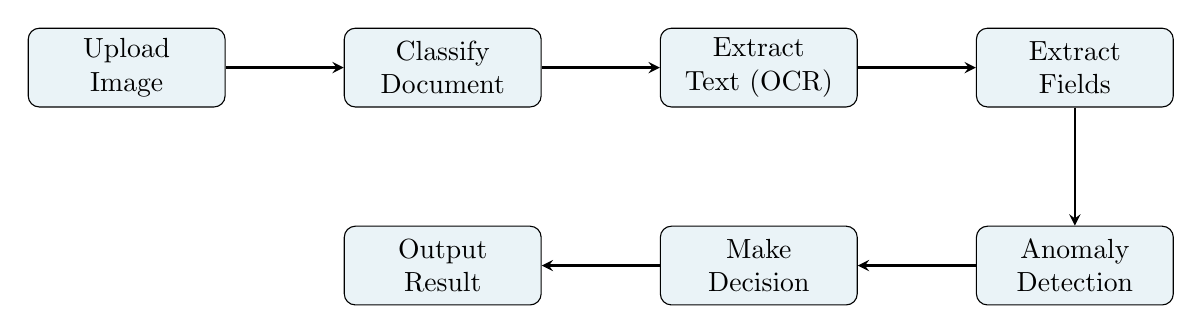
\begin{tikzpicture}[
    node distance=1.5cm,
    box/.style={rectangle, draw, rounded corners, minimum width=2.5cm, minimum height=1cm, align=center, fill=primaryblue!10},
    arrow/.style={->, thick, >=stealth}
]
    \node[box] (input) {Upload\\Image};
    \node[box, right=of input] (classify) {Classify\\Document};
    \node[box, right=of classify] (ocr) {Extract\\Text (OCR)};
    \node[box, right=of ocr] (extract) {Extract\\Fields};
    \node[box, below=of extract] (anomaly) {Anomaly\\Detection};
    \node[box, left=of anomaly] (decision) {Make\\Decision};
    \node[box, left=of decision] (output) {Output\\Result};
    
    \draw[arrow] (input) -- (classify);
    \draw[arrow] (classify) -- (ocr);
    \draw[arrow] (ocr) -- (extract);
    \draw[arrow] (extract) -- (anomaly);
    \draw[arrow] (anomaly) -- (decision);
    \draw[arrow] (decision) -- (output);
\end{tikzpicture}
\end{center}

% ============================================================================
\section{Layer 1: Setup and Dependencies}
% ============================================================================

\subsection{What's Happening Here?}

The first few cells install and import all the tools we need:

\begin{itemize}
    \item \textbf{PyTorch} -- The deep learning framework that runs our neural networks
    \item \textbf{Transformers (HuggingFace)} -- Pre-trained models for vision and language
    \item \textbf{EasyOCR} -- Reads text from images
    \item \textbf{LangGraph} -- Orchestrates the pipeline as a workflow
    \item \textbf{Gradio} -- Creates the web interface
\end{itemize}

\subsection{Key Configuration}

\begin{lstlisting}
DEVICE = 'cuda' if torch.cuda.is_available() else 'cpu'
MODELS_DIR = 'models/'
\end{lstlisting}

\begin{itemize}
    \item Uses GPU if available (much faster), otherwise falls back to CPU
    \item All trained models are saved in the \texttt{models/} folder
\end{itemize}

% ============================================================================
\section{Layer 2: Document Classification}
% ============================================================================

\subsection{Purpose}

Before processing a receipt, we need to verify it actually \textit{is} a receipt. This layer answers: ``Is this image a receipt, invoice, or something else?''

\subsection{How It Works}

We use an \textbf{ensemble} of image classifiers -- multiple models that vote together:

\begin{table}[h]
\centering
\begin{tabular}{lll}
\toprule
\textbf{Model} & \textbf{Type} & \textbf{Role} \\
\midrule
ViT-Tiny & Vision Transformer & Primary classifier \\
ResNet-18 & Convolutional Neural Network & Secondary classifier \\
Stacking Classifier & Meta-learner & Combines both predictions \\
\bottomrule
\end{tabular}
\end{table}

\subsection{Why Ensemble?}

No single model is perfect. By combining multiple models:
\begin{itemize}
    \item ViT is good at understanding overall document structure
    \item ResNet catches fine-grained visual patterns
    \item The stacking classifier learns which model to trust in different situations
\end{itemize}

\subsection{Output}

\begin{lstlisting}
{
    'is_receipt': True,
    'confidence': 0.94,
    'label': 'receipt'
}
\end{lstlisting}

% ============================================================================
\section{Layer 3: OCR (Optical Character Recognition)}
% ============================================================================

\subsection{Purpose}

Convert the image into readable text. This is the ``eyes'' of our system.

\subsection{How It Works}

We use \textbf{EasyOCR} which:
\begin{enumerate}
    \item Scans the image for text regions
    \item Returns each detected word with:
    \begin{itemize}
        \item The text itself
        \item Bounding box coordinates (where on the image)
        \item Confidence score (how sure it is)
    \end{itemize}
\end{enumerate}

\subsection{Retry Logic}

If OCR quality is low (confidence $< 40\%$ or fewer than 3 text regions), the system automatically:
\begin{enumerate}
    \item Increases image contrast
    \item Sharpens the image
    \item Converts to grayscale
    \item Retries OCR (up to 3 attempts)
\end{enumerate}

\subsection{Output Example}

\begin{lstlisting}
[
    {'text': 'STARBUCKS', 'confidence': 0.95, 'bbox': [[10,20], [100,20], ...]},
    {'text': '12/05/2024', 'confidence': 0.88, 'bbox': [[10,50], [80,50], ...]},
    {'text': '$15.99', 'confidence': 0.92, 'bbox': [[10,200], [60,200], ...]}
]
\end{lstlisting}

% ============================================================================
\section{Layer 4: Field Extraction (Ensemble)}
% ============================================================================

\subsection{Purpose}

Turn raw OCR text into structured data. We want to find:
\begin{itemize}
    \item \textbf{Vendor} -- Who issued the receipt (e.g., ``Starbucks'')
    \item \textbf{Date} -- When the transaction occurred
    \item \textbf{Total} -- The amount paid
\end{itemize}

\subsection{The Ensemble Approach}

We use \textbf{4 different strategies} and combine their results:

\begin{table}[h]
\centering
\begin{tabular}{llp{6cm}}
\toprule
\textbf{Strategy} & \textbf{Weight} & \textbf{How It Works} \\
\midrule
LayoutLM & 50\% & Deep learning model that understands document layout \\
Regex & 30\% & Pattern matching (e.g., \texttt{\$XX.XX} for totals) \\
Position & 12\% & Uses location on page (vendor = top, total = bottom) \\
NER & 8\% & Named Entity Recognition for dates and organizations \\
\bottomrule
\end{tabular}
\end{table}

\subsection{LayoutLM Cascade}

LayoutLM is our strongest model. We use a ``cascade'' approach:
\begin{enumerate}
    \item If LayoutLM confidence $\geq 80\%$: Use LayoutLM result directly
    \item Otherwise: Combine all 4 strategies using weighted voting
\end{enumerate}

\subsection{Why This Design?}

\begin{itemize}
    \item LayoutLM is powerful but sometimes uncertain
    \item Regex is fast and reliable for common formats
    \item Position-based rules work well for standard receipts
    \item Combining them gives robust results across different receipt types
\end{itemize}

% ============================================================================
\section{Layer 5: Anomaly Detection}
% ============================================================================

\subsection{Purpose}

Flag suspicious receipts before they're approved. Catches things like:
\begin{itemize}
    \item Unusually high amounts (\$50,000 lunch?)
    \item Missing vendor name
    \item Invalid dates
    \item Suspicious patterns
\end{itemize}

\subsection{The Ensemble}

We combine 4 anomaly detection methods:

\begin{table}[h]
\centering
\begin{tabular}{llp{5cm}}
\toprule
\textbf{Model} & \textbf{Weight} & \textbf{Approach} \\
\midrule
Isolation Forest & 35\% & Finds outliers by isolating unusual points \\
XGBoost & 30\% & Gradient boosting classifier trained on labeled anomalies \\
HistGradientBoosting & 20\% & Handles missing values natively \\
One-Class SVM & 15\% & Kernel-based boundary around normal data \\
\bottomrule
\end{tabular}
\end{table}

\subsection{Features Used}

The models look at:
\begin{itemize}
    \item Amount (and log of amount)
    \item Vendor name length
    \item Whether the date is valid
    \item Number of line items
    \item Time of transaction
    \item Amount per item
    \item Weekend vs weekday
\end{itemize}

\subsection{Output}

\begin{lstlisting}
{
    'is_anomaly': True,
    'score': -0.45,
    'prediction': 'ANOMALY',
    'reasons': ['High amount: $5000.00', 'Missing vendor']
}
\end{lstlisting}

% ============================================================================
\section{Layer 6: LangGraph Workflow}
% ============================================================================

\subsection{Purpose}

Orchestrate all the pieces into a coherent pipeline. LangGraph lets us define the flow as a graph with nodes and edges.

\subsection{The Workflow}

\begin{center}
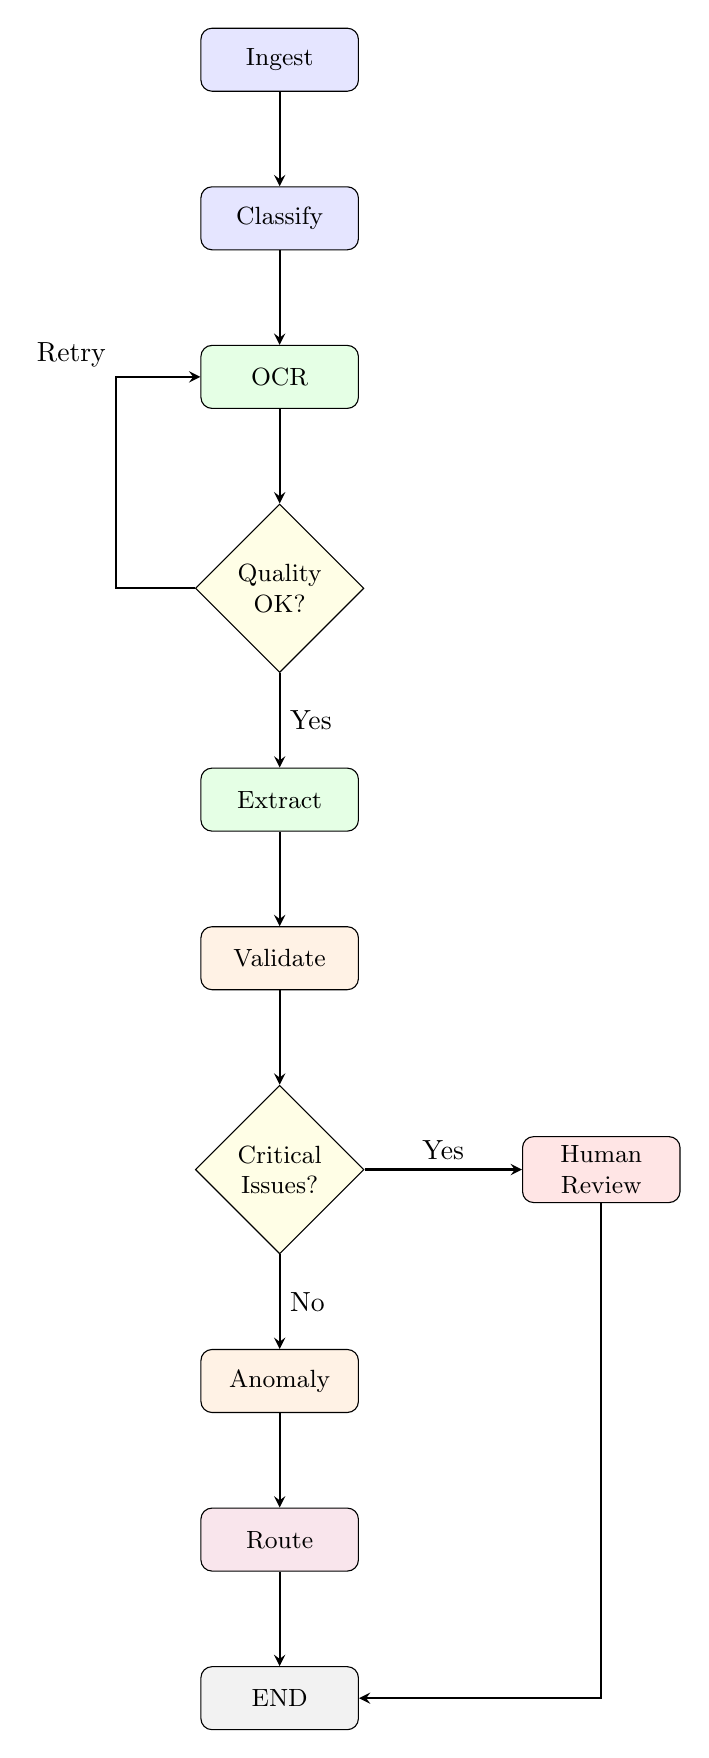
\begin{tikzpicture}[
    node distance=1.2cm,
    box/.style={rectangle, draw, rounded corners, minimum width=2cm, minimum height=0.8cm, align=center, font=\small},
    decision/.style={diamond, draw, minimum width=1.5cm, minimum height=1cm, align=center, font=\small},
    arrow/.style={->, thick, >=stealth}
]
    \node[box, fill=blue!10] (ingest) {Ingest};
    \node[box, fill=blue!10, below=of ingest] (classify) {Classify};
    \node[box, fill=green!10, below=of classify] (ocr) {OCR};
    \node[decision, fill=yellow!10, below=of ocr] (quality) {Quality\\OK?};
    \node[box, fill=green!10, below=of quality] (extract) {Extract};
    \node[box, fill=orange!10, below=of extract] (validate) {Validate};
    \node[decision, fill=yellow!10, below=of validate] (critical) {Critical\\Issues?};
    \node[box, fill=red!10, right=2cm of critical] (review) {Human\\Review};
    \node[box, fill=orange!10, below=of critical] (anomaly) {Anomaly};
    \node[box, fill=purple!10, below=of anomaly] (route) {Route};
    \node[box, fill=gray!10, below=of route] (end) {END};
    
    \draw[arrow] (ingest) -- (classify);
    \draw[arrow] (classify) -- (ocr);
    \draw[arrow] (ocr) -- (quality);
    \draw[arrow] (quality) -- node[right] {Yes} (extract);
    \draw[arrow] (quality.west) -- ++(-1,0) |- node[above left] {Retry} (ocr.west);
    \draw[arrow] (extract) -- (validate);
    \draw[arrow] (validate) -- (critical);
    \draw[arrow] (critical) -- node[above] {Yes} (review);
    \draw[arrow] (critical) -- node[right] {No} (anomaly);
    \draw[arrow] (anomaly) -- (route);
    \draw[arrow] (route) -- (end);
    \draw[arrow] (review) |- (end);
\end{tikzpicture}
\end{center}

\subsection{Key Features}

\begin{itemize}
    \item \textbf{Conditional Branching}: Different paths based on results
    \item \textbf{Retry Logic}: OCR can retry up to 3 times
    \item \textbf{Early Exit}: Non-receipts are rejected immediately
    \item \textbf{Human-in-the-Loop}: Critical issues go to manual review
\end{itemize}

% ============================================================================
\section{Layer 7: Feedback and Learning}
% ============================================================================

\subsection{Purpose}

The system improves over time by learning from human corrections.

\subsection{How Feedback Works}

\begin{enumerate}
    \item User sees the extracted data in Gradio interface
    \item User clicks \checkmark (correct) or \texttimes (wrong)
    \item If wrong, user provides the correct value
    \item Correction is saved to \texttt{feedback\_data/}
\end{enumerate}

\subsection{Batch Fine-Tuning}

After every \textbf{5 corrections}, the system automatically:
\begin{enumerate}
    \item Loads all recent feedback
    \item Fine-tunes the classifier (if document type was wrong)
    \item Fine-tunes LayoutLM (if field extraction was wrong)
    \item Updates the models
\end{enumerate}

\subsection{The FeedbackFineTuner Class}

\begin{lstlisting}
class FeedbackFineTuner:
    def finetune_classifier(self, feedback_data):
        # Actual backpropagation to update classifier weights
        loss.backward()
        optimizer.step()
    
    def finetune_layoutlm(self, feedback_data):
        # Update LayoutLM with corrected field labels
        loss.backward()
        optimizer.step()
\end{lstlisting}

This is \textbf{real neural network training}, not just rule updates.

% ============================================================================
\section{Layer 8: Gradio Interface}
% ============================================================================

\subsection{Purpose}

Provide a user-friendly web interface for:
\begin{itemize}
    \item Uploading receipt images
    \item Viewing extraction results
    \item Providing feedback
\end{itemize}

\subsection{Interface Sections}

\begin{enumerate}
    \item \textbf{Upload Panel}: Drag and drop receipt image
    \item \textbf{Agent Results}: Shows the pipeline's decision (Approve/Review/Reject)
    \item \textbf{OCR Details}: Scrollable section with annotated image showing bounding boxes
    \item \textbf{Classifier Details}: Document type and confidence
    \item \textbf{LayoutLM Details}: Extracted fields with confidence scores
    \item \textbf{Feedback}: Simple \checkmark/\texttimes buttons for each field
\end{enumerate}

\subsection{OCR Visualization}

The annotated image shows:
\begin{itemize}
    \item \textcolor{secondarygreen}{Green boxes}: High confidence ($>80\%$)
    \item \textcolor{warningyellow}{Yellow boxes}: Medium confidence ($50-80\%$)
    \item \textcolor{dangerred}{Red boxes}: Low confidence ($<50\%$)
\end{itemize}

% ============================================================================
\section{Layer 9: Evaluation and Visualization}
% ============================================================================

\subsection{Purpose}

Measure how well each component performs and generate visualizations that are automatically saved and pushed to the repository.

\subsection{Output Directory}

All visualizations are saved to:
\begin{lstlisting}
assets/images/
\end{lstlisting}

This directory is tracked by git, so all team members can access the latest evaluation results.

\subsection{Visualizations Generated}

\begin{table}[h]
\centering
\begin{tabular}{lp{7cm}}
\toprule
\textbf{File} & \textbf{Description} \\
\midrule
\texttt{classification\_confusion\_matrices.png} & Document classifier performance (receipt vs non-receipt) \\
\texttt{anomaly\_confusion\_matrix.png} & Anomaly detector performance (normal vs anomaly) \\
\texttt{classification\_roc\_curves.png} & ROC curve for document classification \\
\texttt{anomaly\_roc\_curves.png} & ROC curve for anomaly detection \\
\texttt{precision\_recall\_curves.png} & Precision-Recall trade-off \\
\texttt{extraction\_strategy\_comparison.png} & Bar chart comparing extraction strategies \\
\texttt{confidence\_distribution.png} & Histogram of model confidence scores \\
\texttt{ensemble\_weights\_viz.png} & Visualization of ensemble voting weights \\
\bottomrule
\end{tabular}
\end{table}

\subsection{Confusion Matrix Details}

The confusion matrices show:

\begin{center}
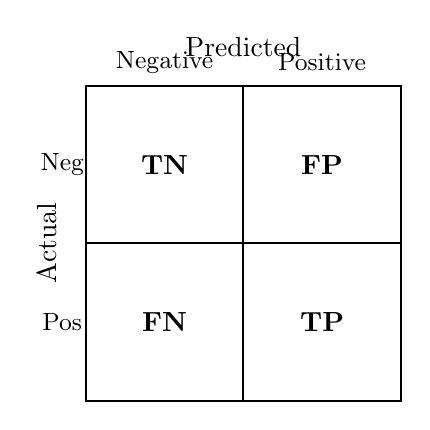
\begin{tikzpicture}
    \draw[thick] (0,0) rectangle (4,4);
    \draw[thick] (2,0) -- (2,4);
    \draw[thick] (0,2) -- (4,2);
    
    % Labels
    \node at (1,3) {\textbf{TN}};
    \node at (3,3) {\textbf{FP}};
    \node at (1,1) {\textbf{FN}};
    \node at (3,1) {\textbf{TP}};
    
    % Axis labels
    \node[rotate=90] at (-0.5,2) {Actual};
    \node at (2,4.5) {Predicted};
    \node at (1,4.3) {\small Negative};
    \node at (3,4.3) {\small Positive};
    \node at (-0.3,3) {\small Neg};
    \node at (-0.3,1) {\small Pos};
\end{tikzpicture}
\end{center}

\begin{itemize}
    \item \textbf{TN} (True Negative): Correctly identified as not anomaly/not receipt
    \item \textbf{TP} (True Positive): Correctly identified as anomaly/receipt
    \item \textbf{FP} (False Positive): Incorrectly flagged (Type I error)
    \item \textbf{FN} (False Negative): Missed detection (Type II error)
\end{itemize}

\subsection{Auto-Push with GitPusher}

The \texttt{GitPusher} class automatically commits and pushes visualizations:

\begin{lstlisting}
class GitPusher:
    def push_file(self, filepath, message=None):
        # Adds, commits, and pushes a single file
        
    def push_all(self, filepaths, message=None):
        # Batches multiple files in one commit
\end{lstlisting}

\textbf{How it works:}
\begin{enumerate}
    \item When \texttt{save\_figure()} is called, the image is saved to \texttt{assets/images/}
    \item GitPusher automatically runs \texttt{git add}, \texttt{git commit}, \texttt{git push}
    \item Commit message includes timestamp for tracking
\end{enumerate}

\subsection{EnsembleEvaluator Class}

The main evaluation class provides these methods:

\begin{table}[h]
\centering
\begin{tabular}{lp{6cm}}
\toprule
\textbf{Method} & \textbf{Output} \\
\midrule
\texttt{plot\_anomaly\_confusion\_matrix()} & Confusion matrix for anomaly detection \\
\texttt{plot\_classification\_confusion\_matrices()} & Confusion matrix for document classification \\
\texttt{plot\_classification\_roc\_curves()} & ROC curves with AUC scores \\
\texttt{plot\_precision\_recall\_curves()} & PR curves for imbalanced evaluation \\
\texttt{plot\_extraction\_strategy\_comparison()} & Bar chart of extraction strategy performance \\
\texttt{push\_all\_figures()} & Batch push all saved figures to GitHub \\
\bottomrule
\end{tabular}
\end{table}

\subsection{Viewing Results}

After running evaluation cells:

\begin{enumerate}
    \item Figures appear in Colab output
    \item Simultaneously saved to \texttt{assets/images/}
    \item Automatically pushed to GitHub
    \item Team can view at: \texttt{github.com/RogueTex/StreamingDataforModelTraining/assets/images/}
\end{enumerate}

\subsection{Manual Push (if auto-push fails)}

If running locally or auto-push fails in Colab:

\begin{lstlisting}[language=bash]
cd /path/to/StreamingDataforModelTraining
git add assets/images/*.png
git commit -m "Add evaluation visualizations"
git push
\end{lstlisting}

% ============================================================================
\section{File Structure}
% ============================================================================

\begin{lstlisting}
StreamingDataforModelTraining/
|-- NewVerPynbAgent.ipynb    # Main notebook with all code
|-- models/
|   |-- rvl_classifier.pt    # Document classifier
|   |-- layoutlm_extractor.pt # Field extraction model
|   |-- anomaly_detector.pt   # Anomaly detection model
|-- feedback_data/            # Stored user corrections
|-- assets/images/            # Evaluation visualizations (auto-pushed)
|-- data/                     # Training data (if any)
|-- docs/                     # Documentation (this file)
\end{lstlisting}

% ============================================================================
\section{Quick Reference: Key Classes}
% ============================================================================

\begin{table}[h]
\centering
\begin{tabular}{lp{8cm}}
\toprule
\textbf{Class} & \textbf{Purpose} \\
\midrule
\texttt{DocumentClassifier} & Classifies images as receipt/non-receipt \\
\texttt{ReceiptOCR} & Extracts text from images using EasyOCR \\
\texttt{LayoutLMFieldExtractor} & Uses LayoutLM to extract structured fields \\
\texttt{EnsembleFieldExtractor} & Combines 4 strategies for robust extraction \\
\texttt{ReceiptAnomalyDetector} & Flags suspicious receipts \\
\texttt{EnsembleAnomalyDetector} & Combines 4 anomaly detection methods \\
\texttt{FeedbackFineTuner} & Retrains models from user feedback \\
\texttt{GitPusher} & Auto-pushes visualizations to GitHub \\
\texttt{EnsembleEvaluator} & Generates confusion matrices, ROC curves, etc. \\
\bottomrule
\end{tabular}
\end{table}

% ============================================================================
\section{Running the Pipeline}
% ============================================================================

\subsection{In Google Colab}

\begin{enumerate}
    \item Open \texttt{NewVerPynbAgent.ipynb} in Colab
    \item Run cells 1-4 (Setup and Dependencies)
    \item Run cells 5-30 (Model Loading)
    \item Run the Gradio cell (cell 57)
    \item Click the Gradio link to open the interface
\end{enumerate}

\subsection{Processing a Receipt}

\begin{enumerate}
    \item Upload an image
    \item Wait for processing (usually 2-5 seconds)
    \item Review the results in each accordion section
    \item Provide feedback if any field is wrong
    \item After 5 corrections, fine-tuning triggers automatically
\end{enumerate}

% ============================================================================
\section{Troubleshooting}
% ============================================================================

\begin{table}[h]
\centering
\begin{tabular}{lp{8cm}}
\toprule
\textbf{Issue} & \textbf{Solution} \\
\midrule
``CUDA out of memory'' & Reduce batch size or use CPU \\
OCR returns empty & Check image quality, try preprocessing \\
LayoutLM slow & Normal on CPU; use GPU for speed \\
Git push fails & Check Colab has repo access; run manually \\
Low confidence scores & Image may be blurry or unusual format \\
\bottomrule
\end{tabular}
\end{table}

% ============================================================================
\section{Future Improvements}
% ============================================================================

\begin{itemize}
    \item Add support for multi-page receipts
    \item Implement active learning for smarter feedback sampling
    \item Add support for different languages
    \item Integrate with expense management systems
    \item Add receipt categorization (food, travel, office supplies)
\end{itemize}

\end{document}
